\begin{savequote}[65mm]
%\begin{displayquote}
``Humanistic Intelligence [HI] is intelligence that arises because of a human being in the feedback 
loop of a computational process, where the human and computer are inextricably intertwined. When a 
wearable computer embodies HI and becomes so technologically advanced that its intelligence 
matches our own biological brain, something much more powerful emerges from this synergy that 
gives rise to superhuman intelligence within the single `cyborg' being."
%\end{displayquote}
\qauthor{-- Marvin Minsky, Ray Kurzweil, \\and Steve Mann~\cite{minsky2013society} }
\end{savequote}

\chapter{Introduction}
Fundamentally, human is ``bandwidth-limited". We can only see so far or resolve so much information 
%-- the human eye has an angular resolution of approximately 1 arcminute or 1/60 degree
\cite{ophthalmology3rd}. We can only sense so much information 
%-- human can only perceive  physical stimuli above a certain threshold
and we can only detect a limited spectrum of light and sound~\cite{laming1986weber}. We can only process information at a limited rate~\cite{martin2009thermodynamics}.
%%of about 30 to 100 bits/s%

To overcome these limitations, we have created many tools and 
inventions that revolutionized the way we ``see'' and understand this world. The first invention of 
eyeglasses (or glasses) -- a pair of plastic or glass lenses which had a specific prescription and was 
mounted in a frame that held them in front of a person's eyes -- was first documented in the 12th 
century~\cite{rosen1956invention} and was primarily used to correct for refractive errors. Today, 
specialized eyeglasses are also used for purposes such as magnifying an object of interest during a 
surgical procedure and protecting our eyes in more dangerous settings including welding or high-
power laser procedures. Modern advancements in technology, particularly in processing power and 
sensor capability, have allowed us to overcome our own limitations by enabling the creation of novel 
devices that can receive and process information much faster and in more versatile ways than human. 
It is clear that such advancements have surpassed the pace of our own biological evolution. This 
dissertation presents the design of a digital form of eyeglasses that can significantly improve our 
vision, extend our sensory capabilities, and create a new form of human computer interaction that is 
truly human-centric. 

\section{Introduction to `Digital' Eye Glass}
\label{introdigitalglass}

In the 1960s, Ivan Sutherland first described the concept of a head-mounted three dimensional 
display system which presents the user with a virtual, perspective-corrected, image that changes with 
respect to the user's head movement~\cite{sutherland1968head}. The apparatus, as shown in 
Fig.~\ref{ivanfullsetup}, was cumbersome and had to be mounted in the ceiling with a mechanical arm 
due to its weight and size. The display can only render a transparent ``wire frame" line drawing and no 
additional user inputs, such as hand gesture, can be provided. Most importantly, this concept was not 
ubiquitously adopted at the time because the rendered content does not provide information in a 
meaningful way with the real world. Despite all these shortcomings, this initial prototype inspired 
further research based on head-mounted systems for human-computer interaction 
~\cite{feiner1993knowledge,feiner1997touring,caudell1992augmented,stoakley1995virtual,billinghurst2015rapid,kato1999marker,billinghurst2002augmented}.


\begin{figure*}[t]
\centering
\begin{subfigure}[t]{1.75in}
  \centering
  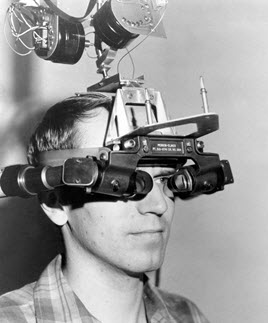
\includegraphics[height=2.0in]{ch1/figures/sutherland/3.jpeg}
  \caption{}
  \label{ivansetup1}
\end{subfigure}
\begin{subfigure}[t]{2.6in}
  \centering
  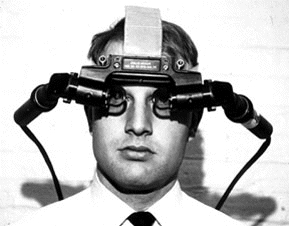
\includegraphics[height=2.0in]{ch1/figures/sutherland/2.jpeg}
  \caption{}
  \label{ivansetup2}
\end{subfigure}
\begin{subfigure}[t]{1.4in}
  \centering
  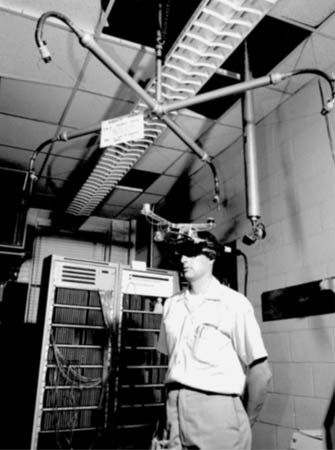
\includegraphics[height=2.0in]{ch1/figures/sutherland/1.jpeg}
  \caption{}
  \label{ivansetup3}
\end{subfigure}
\caption{(a) The head-mounted three dimensional display system, also known as ``The Sword of 
Damocles", worn by Donald L. Vickers, one of Ivan Sutherland's students~\cite{sutherland1968head}. (b) The head-mounted 
display and the optics with mini-CRT. A stereoscopic pair of computer-generated images were 
projected to the user's eyes through the half-silvered mirrors. The apparatus allows the user to see 
both the real world and virtual images at the same time and perform simple interaction with head 
motion~\cite{sutherland1968head}. (c) The mechanical, ultrasonic head position sensors, which were mounted in the ceiling and 
were designed at the MIT Lincoln Laboratory by Charles Seitz and Stylianos Pezaris, were used to 
retrieve the head position and orientation in real time~\cite{sutherland1968head}.}
\label{ivanfullsetup}
\end{figure*}

\subsection{History of Wearable Computing}
In 1974, Mann invented the S.W.I.M. (Sequential Wave Imprinting Machine) which included a special kind of lock-in amplifier and wearable computer that could sweep for surveillance devices, and display the results of this "bug sweeping" activity on a linear array of sequentially illuminated light sources\cite{mann1992wavelets, impulse, mann2014sightfield, kineveillance}.

In the 1980s, the idea of a Digital Eye Glass, Wearable Computer (WearComp) was introduced by 
Mann~\cite{mannaaai361, mann1994mediated, mannwyckofftr, aimone2003eyetap} as a 
practical realization of humanistic computing~\cite{mann2001wearable, 
intelligentimageprocessing,presenceconnect,mann260}, and an extension of human capability for our 
everyday life. The WearComp project significantly transformed the way we think about wearable 
computers by proposing a framework for the integration of human into the signal processing path, 
thus creating the notion of humanistic intelligence~\cite{mann2001wearable, 
intelligentimageprocessing}. This work has important implications extending beyond the engineering 
challenges into the broader social implications, such as the concept of \emph{sousveillance}
~\cite{mann2002sousveillance, mann2004sousveillance, mann2006cyborglogging}) as opposed to 
the conventional notion of \emph{surveillance}, which emerge as a result of this new form of 
ubiquitous, wearable computing. 

\begin{figure}[htb]
\center
 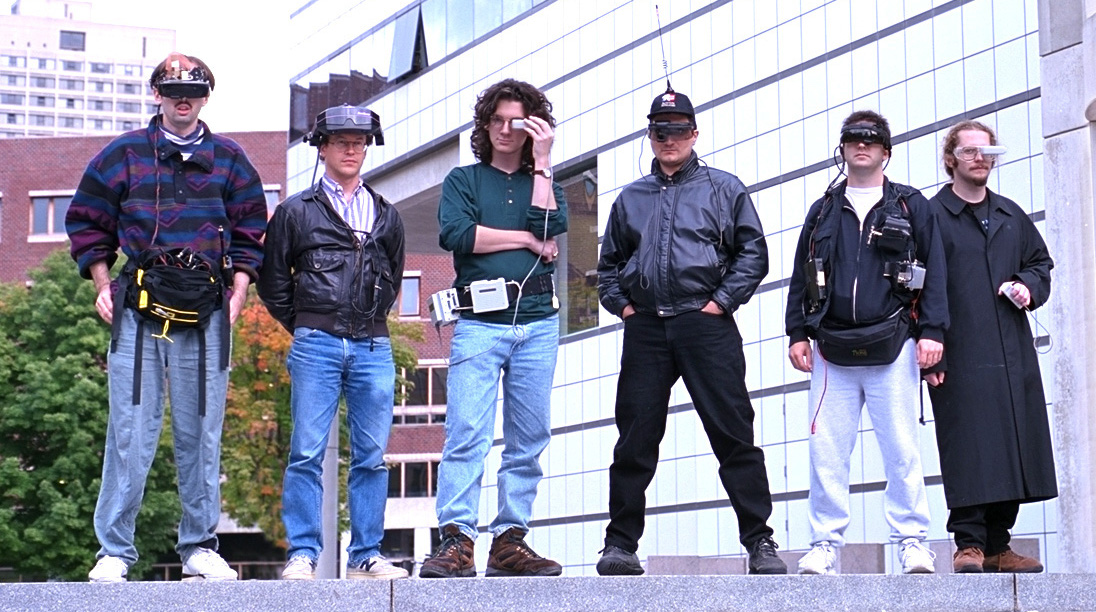
\includegraphics[width=5.5in]{ch1/figures/cyborgs.jpg}
 \caption{This picture showed the early members who experimented with the wearable computer and applications at MIT Media Lab in 1996. Particularly, individuals were wearing computers which were connected wirelessly to create the 'safety net', an application which allows users to provide crime watching by sharing their individual image streams~\cite{mann1997smart}. Image source: \url{http://www.wearcam.org/computing.html/imageinfo.html}. 
 }
 \label{fig:cyborgs}
\end{figure}

Furthermore, Thad Starner designed the wearable computer called ``The Lizzy'' based on the PC/104 form factor~\cite{starner1997augmented} in 1996. By continuously wearing computers in everyday life, a set of novel wearable applications such as``Augmented Memory"~\cite{starner1997augmented} which automatically augment based on the context of the user and augmented reality applications which provide face detection and finger tracking~\cite{rhodes1997wearable} were emerged.  These applications, however, often suffers from the lack of high fidelity display for information displays, the lack of robust sensors for recognizing gestures, and the lack of processing power and tracking capability to be truly practice for daily use.

%Then Feiner\~cite{}

%Later in 1994, Mann then first transmitted images from his head-mounted camera system to the world wide web. See Figure~\ref{fig:mannglass} (c-d).

%These merging applications fundamentally require a better sensing technology, and algorithm to capture, to display with higher dynamic range display, and to process information around user's environment in real-time to provide a meaningful purpose for the uses.


\subsection{Digital Eye Glass}
%problem statement.
\begin{figure}[htb]
\center
 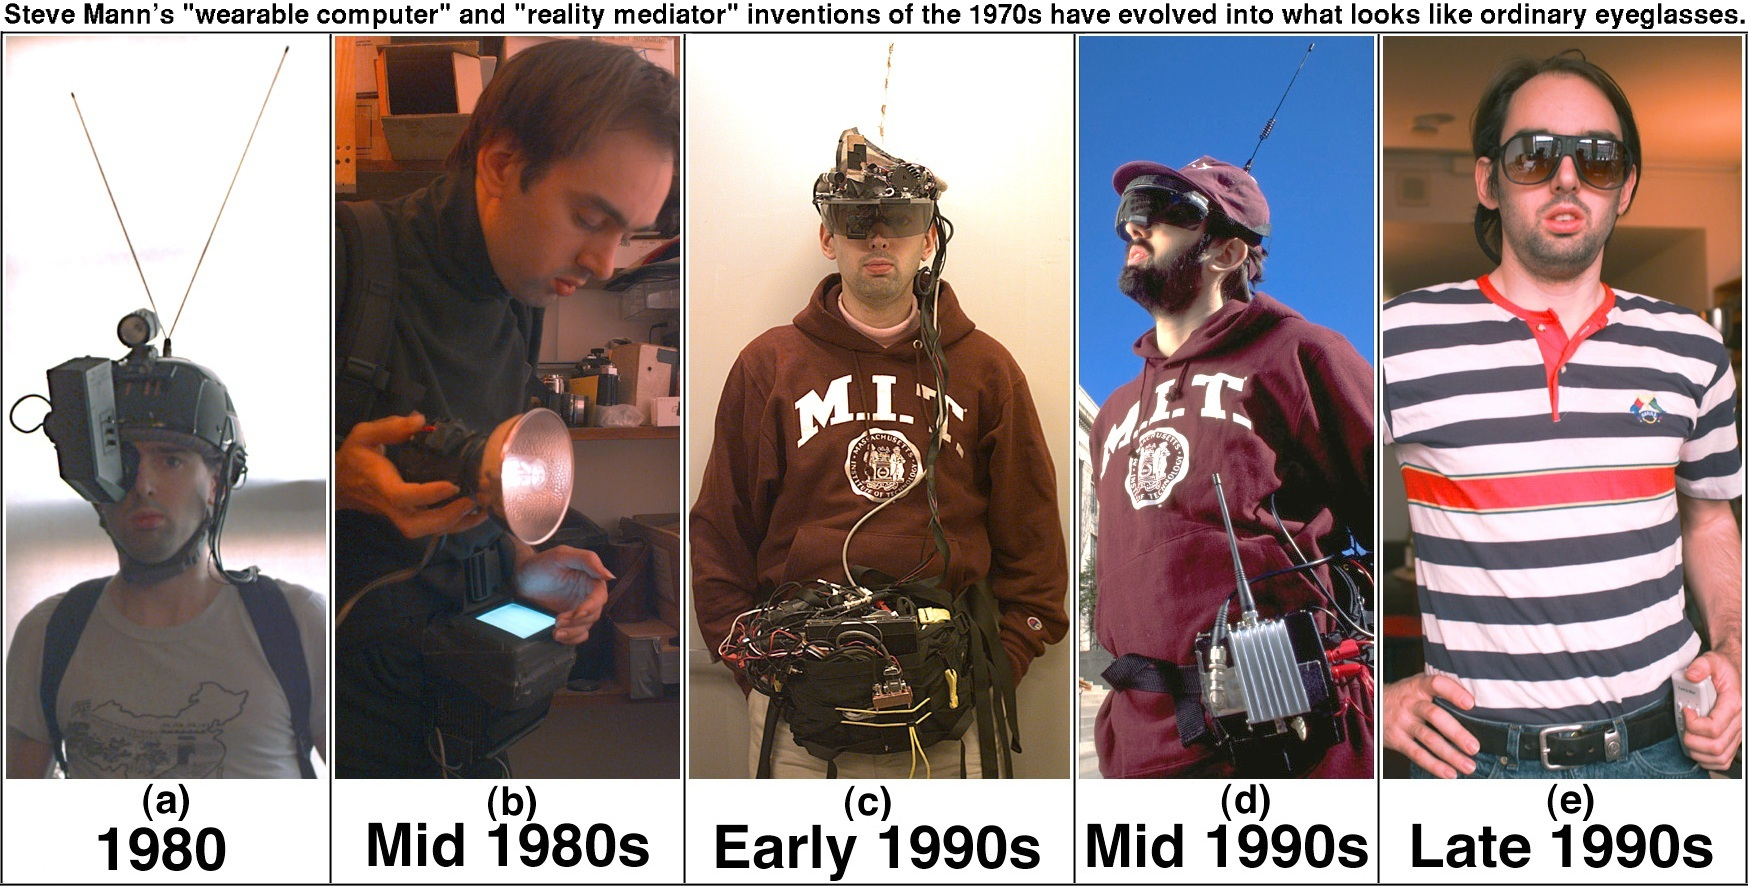
\includegraphics[width=5.5in]{ch1/figures/steve5.jpeg}
 \caption{(a) Mann's original work for the ``photographer's assistant" application. The early prototype 
of the WearComp is a backpack-based computer system with a right eye display mounted on a 
helmet. Two radio wireless antennas run at different frequencies for full-duplex radio link for voice, 
video, and data communication~\cite{mann1994mediated}. (b) Prototypes of input devices with the WearComp 
project. An electronic flash light and a waist-mounted display are shown. (c-d) The world's first portable or 
wearable weblogging WearComp prototypes for Reality Mediator applications. The devices enable 
remote collaboration and the ability to alter the wearer's perception around the environment through 
Mediated Reality~\cite{mann1994mediated}. (e) A WearComp prototype which fits within the form 
factor of ordinary eyeglasses. Such a prototype is suitable for everyday usage in the society. The 
apparatus consists of a UNIX-based computer concealed under ordinary clothing, and a display and 
camera that fit within the eyeglasses~\cite{intelligentimageprocessing}.}
 \label{fig:mannglass}
\end{figure}

The EyeTap Digital Eye Glass functions as a seeing aid to help with specific tasks such as electric arc 
welding as well as in general day-to-day tasks, through a general-purpose computer in the form of 
eyeglasses or simply \emph{eye glass}~\cite{intelligentimageprocessing}. The EyeTap device causes 
the eye itself to, in effect, function as if it were both a camera and a display. Such a design gives the 
wearer the appearance of having a glass eye (See Fig.~\ref{fig:eyetap_mann_black}) so this 
phenomenon has become known as the ``Glass Eye'' effect~\cite{mann260}. 

\begin{figure}
  \center
  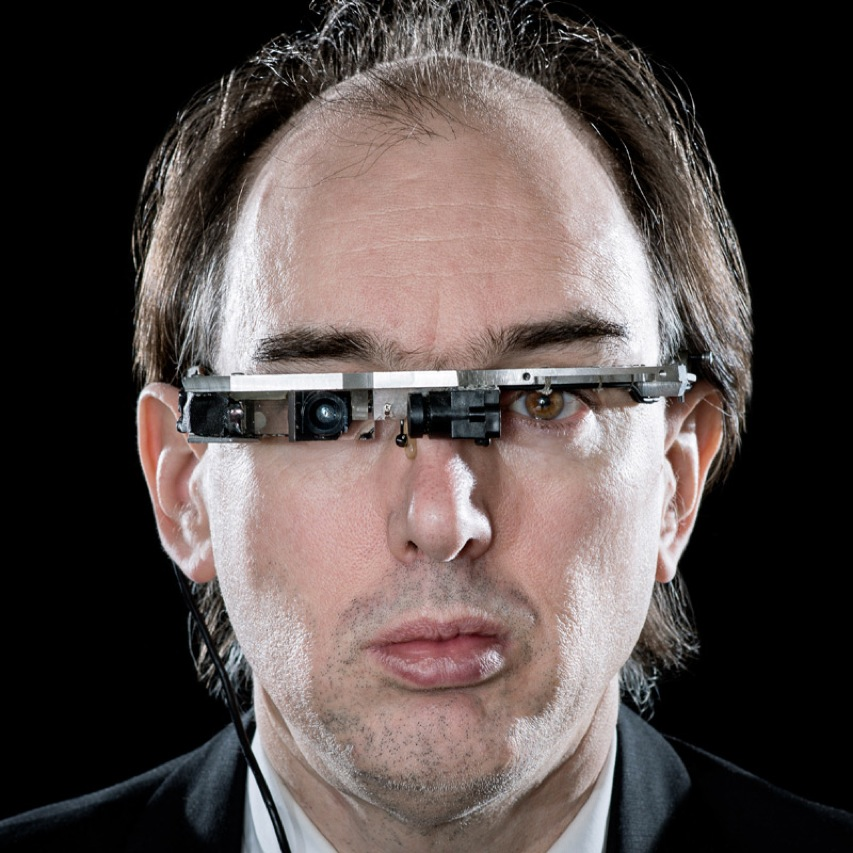
\includegraphics[width=3.0in]{ch1/figures/eyetap.jpg}
  \caption{The EyeTap system. The eye itself is, in effect, both the camera and display~\cite{mann2013steve}.}
  \label{fig:eyetap_mann_black}
\end{figure}

Thus EyeTap is sometimes called the ``Glass Eye'', as well as the ``Eye Glass'', or simply ``Glass''. 
Note the term ``Glass'' singular, rather than ``Glasses'' plural, has been widely used to describe this 
invention. Example applications running on the Glass included the Visual Memory 
Prosthetic~\cite{mannaaai361} which helps people, especially the elderly or those with visual 
impairment, to remember names, faces and other information in our environment. The EyeTap device 
can also service as a wayfinding tool with a GPS navigation system that goes beyond what is possible 
with traditional analog optical glasses. 

This apparatus helps the wearer see better in their everyday life, while also functioning as an interface 
for a general-purpose wearable computer. Today, companies such as Google are investing in the 
development of digital eyeglasses, such as Google Glass\footnote{\url{https://developers.google.com/
glass/}} that shares a number of features seen in the early EyeTap system. More recently, other 
companies such as Microsoft, Meta, and Intel have released various developer kits (e.g., 
Hololens\footnote{\url{https://www.microsoft.com/microsoft-hololens/en-us}} and Meta 
2\footnote{\url{https://www.metavision.com/}}) which provide a platform for the community to develop 
Aug-mediated Reality applications~\cite{mann1994mediated}.

%Metaveillance/Metavision is the veillance of veillance (vision of vision), i.e. the sensing of sensors and the sensing of their capacity to sense. In the same way that a meta-conversation is a conversation about conversations, meta data is data about data, etc., metavision is the vision of vision. Metaveillance/metavision, when combined with abakography, results in a phenomenological augmented reality that makes real-world physical phenomena visible~\cite{toposculpting_ccece2014}.

Mann's metaveillance apparatus evolved toward a general-purpose wearable computer with wearable camera and display, equipped with gesture-sensing capabilities, so that it responds to the wearer's own self-gestures (e.g. it can see the wearer's own hands and thus create an interactional space in which the main design tools that the user uses are his or her own hands)~\cite{mannieeecomputer}. Mann's coined the term "Synthetic Synesthesia of the Sixth Sense", often abbreviated "SixthSense", to describe these gesture-based wearable computer systems~\cite{cyborg, geary2002body}.

Mann, Huang, Janzen, Lo, and others, added 3D depth-sensing capability to Sixth Sense in 2010, and used the Sixth Sense system to assist the blind and visually impaired~\cite{mann2011blind}.

In 2012, Mann and Gribetz joined forces in a collaboration that combined Mann's Sixth Sense and Metaveillance/Metavision technologies toward the production of a commercial product (patent written in 2012 and filed on January 3, 2013~\cite{patentmetadepth}).

By further adding the Toposculpting invention, a combination of three important technologies resulted:
1. Sixth Sense;
2. Metaveillance/Metavision;
3. Toposcuplting (topological sculpting), i.e. using 3D gesture-recognition for computational lightpainting by way of wearable computational photography for abakographic user-interfaces~\cite{patentmetabakography}. Subsequently, Gribetz (CEO and founder), Mann (Chief Scientist), and Lo (Chief Technology Officer and co-founder) joined forces to found the new company Meta Company, and introduce to the world the concept of Extramissive Spatial Imaging Glass~\cite{gribetz2014extramissive}. 

\section{A Theory of Glass: Background information}
%{\bf Note to reviewers:}
%{\em This section presents a review of Generations 1-4 of Digital Eye Glass.
%This section appears in another paper submission to i-Society 2013.
%If both papers are accepted for publication, the overlap will be
%eliminated to avoid double-publishing of this section.}

Digital Eye Glass is a wearable computer system that reconfigures the eye(s)
for Aug-mediated Reality, i.e. a visual reality that can be augmented or
deliberately diminished to, for example, help people see better by enhancing the image through 
magnification or contrast improvement in their everyday life through a `visual 
filter'~\cite{mann1994mediated}. 
In this sense, this is originally referred to as ``Glass'' rather than ``Glasses'' (the more common plural 
form of the word), as shown in Fig.~\ref{fig:glass}. 

\begin{figure}
\center
  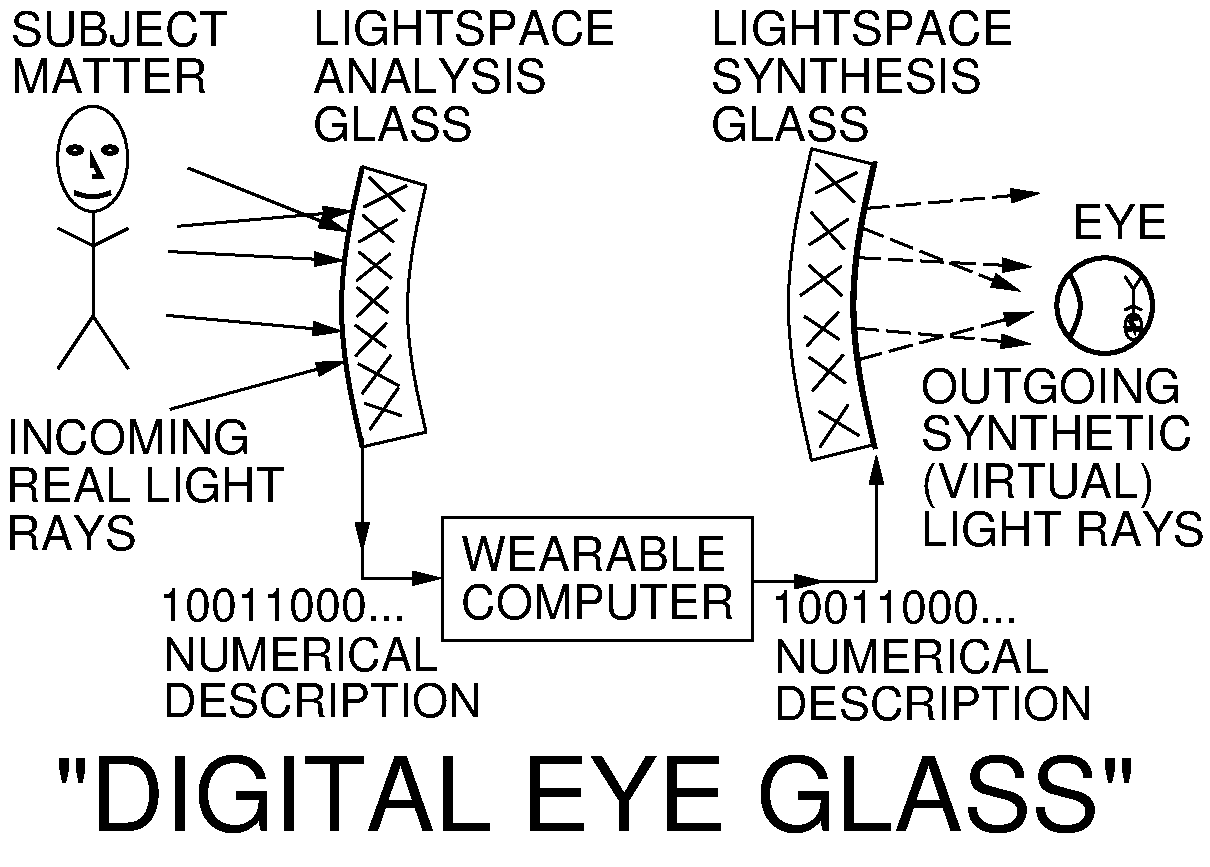
\includegraphics[width=3.5in]{ch6/figs/Glass.pdf}
  \caption{A theory of Glass: rays of eyeward bound light are captured
           by an ``analysis glass'', then processed by the wearable computer
           in the glass system, and then re-synthesized by a
           ``synthesis glass''~\cite{mann2013freeglass}.}
  \label{fig:glass}
\end{figure}

Rays of eyeward-bound light strike a ``Lightspace Analysis Glass'' (which need not necessarily be flat, 
and is therefore depicted as being curved), are converted to numbers which may then be processed 
by the wearable computer. The resulting numbers are fed to a ``Lightspace Synthesis Glass'' to be 
converted back into light.  This allows the wearable computer to become a visual intermediary, to, for 
example, diminish the bright areas
of the Subject Matter, and Augment/Mediate the bright areas, before resynthesizing the rays of light 
into the Eye, as shown in Fig~\ref{fig:glass}.

\subsection{Generation-1 Glass:}
The original approximation prototype of this glass was built in 1978, using a television camera as the 
``Lightspace Analysis Glass'' a miniature glass cathode-ray tube display as the ``Lightspace Synthesis 
Glass'' (over the right eye), and some electric circuits as the wearable computer, as shown in 
Fig.~\ref{fig:mannglass} (a).

Because the camera was located beside the eye, the long-term effects after many hours of wearing 
the apparatus consisted of an adaptation to this strange way of seeing, and the adaptation persisted 
after the removal of the apparatus~\cite{mann1994mediated}. 

Others found similar effects. For example, George Stratton in his work of 1896, with an upside-down 
glass
(done optically rather than electrically), found that it took him about a week to adapt to seeing with 
mediated vision, and about one full day to return to seeing properly (normally) after removing the 
glass~\cite{stratton1897vision}.

It is observed that mappings that deviate moderately from what the unaided eye saw, were harder to 
``forget'' than mappings that were either closer to or further from what the unaided eye saw.  The 
camera must, in effect be the eye itself, if we were to avoid the strange ``flashback'' effects and other 
fatigues due to accommodation to the Generation-1 Glass ~\cite{schor1987fatigue}.

\begin{figure}
  \center
  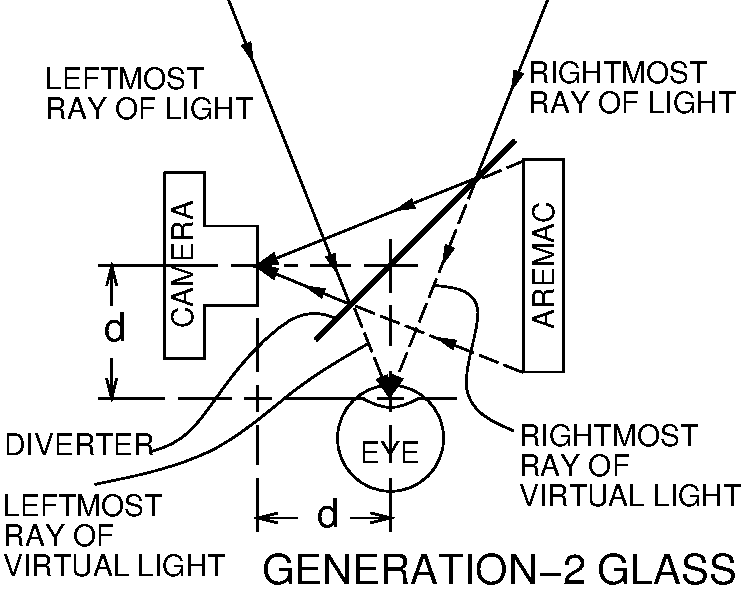
\includegraphics[width=3.5in]{ch6/figs/GlassGen2.pdf}
  \caption{Generation-2 Glass: The eye itself is, in effect, both the camera
           and display.  This eliminates the undesirable ``flashback'' effects
           that otherwise arise from long-term usage~\cite{mann2013freeglass}.}
  \label{fig:gentwo}
\end{figure}

\subsection{Generation-2 Glass}
Generation-2 Glass is developed in which Rays of eyeward-bound light were diverted into a camera 
system that feeds to the wearable computer which then drives an Lightspace Synthesis 
Glass~\cite{mann2001aremac}). In this way, rays of light that would have entered the unaided eye are 
collinear with rays of light presented by the Gen-2 Glass (Fig~\ref{fig:gentwo}). This setup addressed 
the ``flashback'' effects in Gen-1 Glass by carefully aligning the real-world and mediated content. 
However, it does not provide any real world tracking or refocusing capability, and assumes that the 
user is looking into the far range only.

\subsection{Generation-3 Glass}
Particularly in monocular systems, when one eye is focused on a display, and the other is focused on 
direct
``reality'', there is a difference in focal distance between the two eyes. To overcome this problem, 
Generation-3 Glass was developed using a special display called an 
``aremac''~\cite{mann2001aremac} which has the ability to present visual information at an apparent 
focal distance that can be controlled by the wearable computer. The computer senses where objects 
are in 3-dimensional space, and makes an inference as to what range of focal distances the non-
glass-eye can focus to. Information is presented to the glass-eye in this same focal range, which is 
automatically updated several times per second.

\begin{figure}
  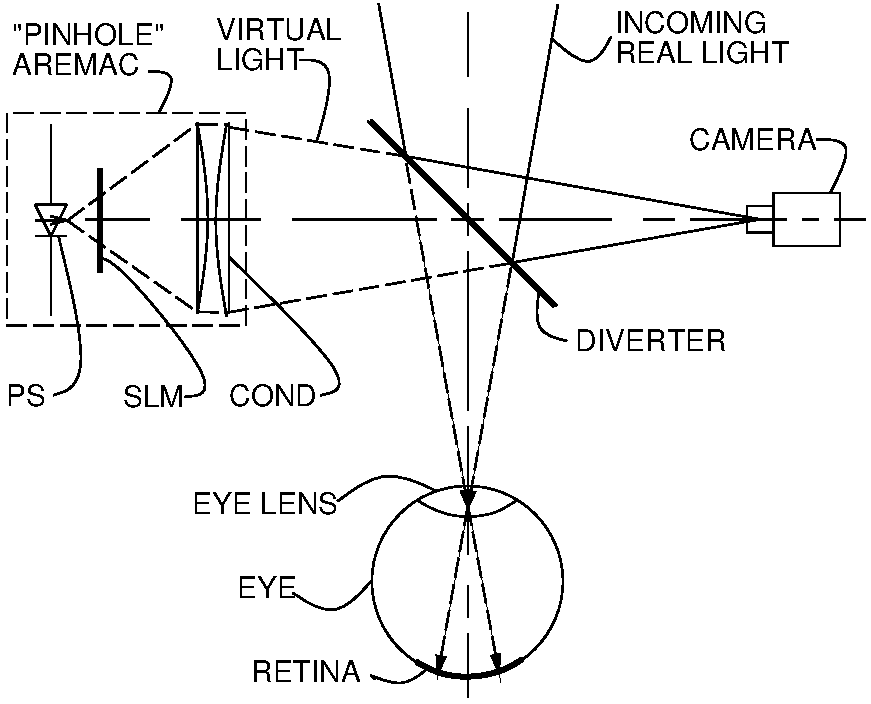
\includegraphics[height=2.4in]{ch6/figs/GlassGen4a.pdf}
  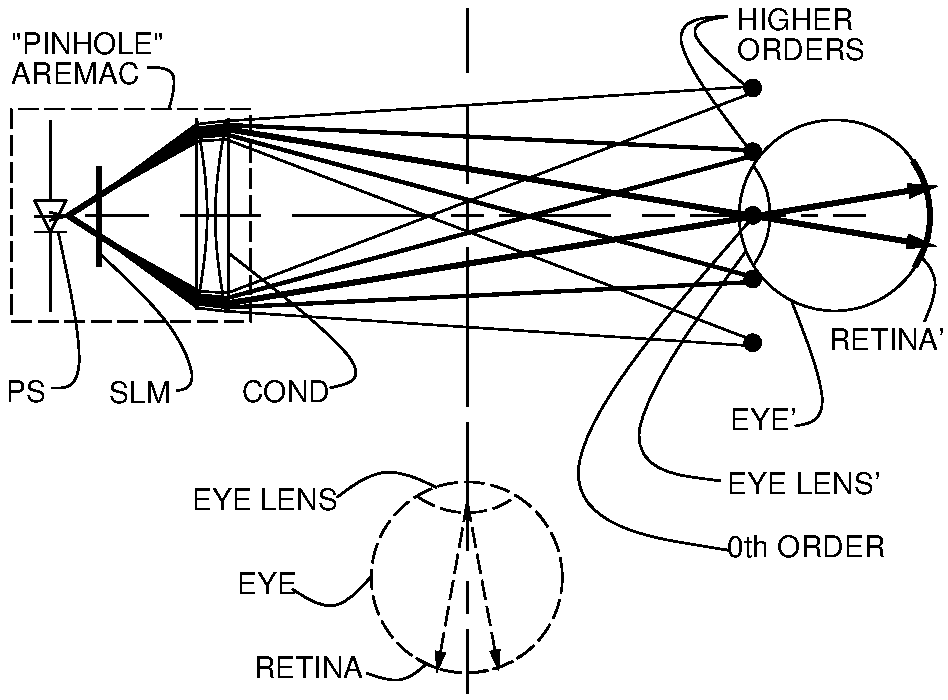
\includegraphics[height=2.4in]{ch6/figs/GlassGen4b.pdf}\\
  {\sffamily \large GENERATION-4 GLASS}\\
  \caption{Generation-4 Glass uses a laser light source to achieve
           infinite depth-of-focus to bypass the eye's lens.  Therefore,
           the glass-eye is not presented with information at any particular
           focal distance, leaving it free to focus at whatever distance the
           other eye is focused to~\cite{mann2013freeglass}.}
  \label{fig:genfour}
\end{figure}

\subsection{Generation-4 Glass}
While looking at objects in various focal planes, such as looking at a distant object through a nearby 
screen or chainlink fence, some problems remained with the Generation-3 Glass. Often, this may 
create eye fatigue due to the accommodation and vergence issue~\cite{hoffman2008vergence}. 

These problems were overcome with the Generation-4 Glass.  The Gen-4 Glass uses a laser light 
source
with a spatial light modulator, and related apparatus, to attain an infinite depth-of-focus, so that the 
displayed information is always in focus regardless of where the eye focuses. The laser EyeTap 
bypasses the lens of the glass-eye and forms an image directly on the retina. In this way, the Gen-4 
Glass does not cause the eye to focus at any particular distance, leaving it free to focus where the 
non-glass eye is focused (Fig~\ref{fig:genfour}).

Generations~2 to~4 Glass were known as ``EyeTap Digital Eye Glass''~\cite{edeg} (the word ``Glass'' 
appears in its singular form, not plural, i.e., ``Eye Glass'' not ``Eye Glasses'').

The result was a natural experience with zero eye strain and could be worn continuously many hours 
a day for many years. The Generation-4 Glass prototype was presented in 1999 and described in 
detail in 2001~\cite{intelligentimageprocessing} (Fig.~\ref{fig:mann_glass_google} (leftmost)).
% (the cover, first page, and pages 31-32) of Abilities Magazine, Issue 69, Winter 2006.

\begin{figure}
  \centering
  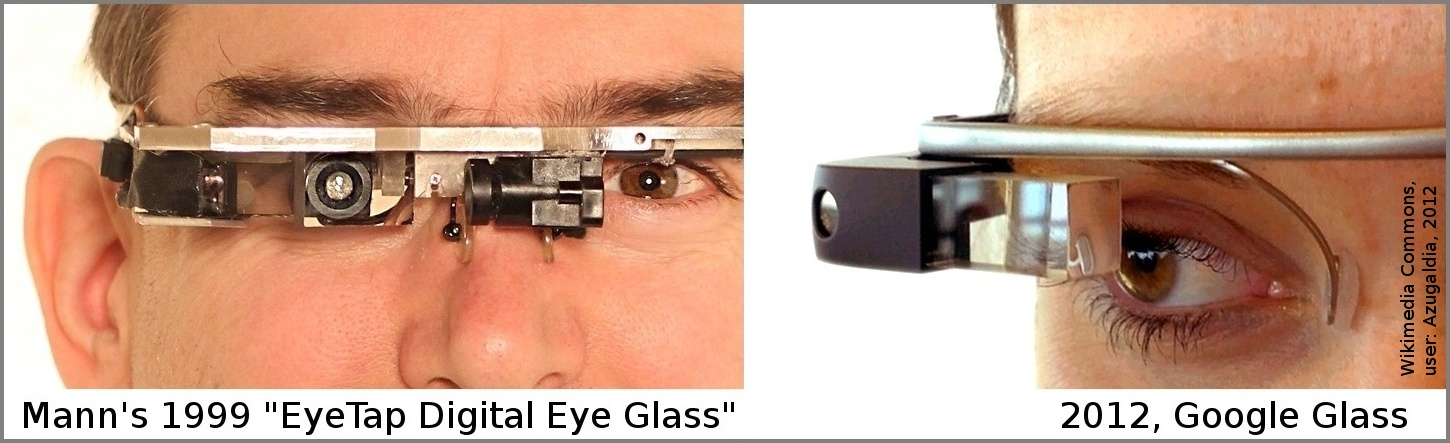
\includegraphics[width=5.5in]{ch6/figs/MannGlass_GoogleGlass_with_narrowborder_closer.jpg}\\
  \caption{Leftmost: Generation-4 Glass completed in 1999.
         {\bf The eye itself is the camera exactly!}
         That is why the ``Digital Eye Glass'' is also known as
         the ``GlassEye'' (The eye looks exactly like a camera lens).  This
         eliminates long-term dizziness, vertigo, and flashback effects
         that can otherwise persist long after the Glass is removed.
         Rightmost: Google Glass, 2012, where the camera being positioned to one
         side of the eye makes it a Generation-1 Glass, subject to some
         of the problems discovered earlier on ~\protect\cite{mann2013vision,mann2013freeglass}.
        }
  \label{fig:mann_glass_google}
\end{figure}

\subsection{Generation-5 Glass}
To further extend on the earlier work, Generation-5 is defined as being bi-directional in its light sensing 
and light output capabilities.  In this way, the Gen-5 Glass senses both the scene in front of the wearer 
as well as the wearer's
own eyes; it also illuminates both the wearer's eyes and the scene in front of the wearer 
(Fig~\ref{fig:genfive})

%\begin{figure}
\begin{figure}
  \centering
  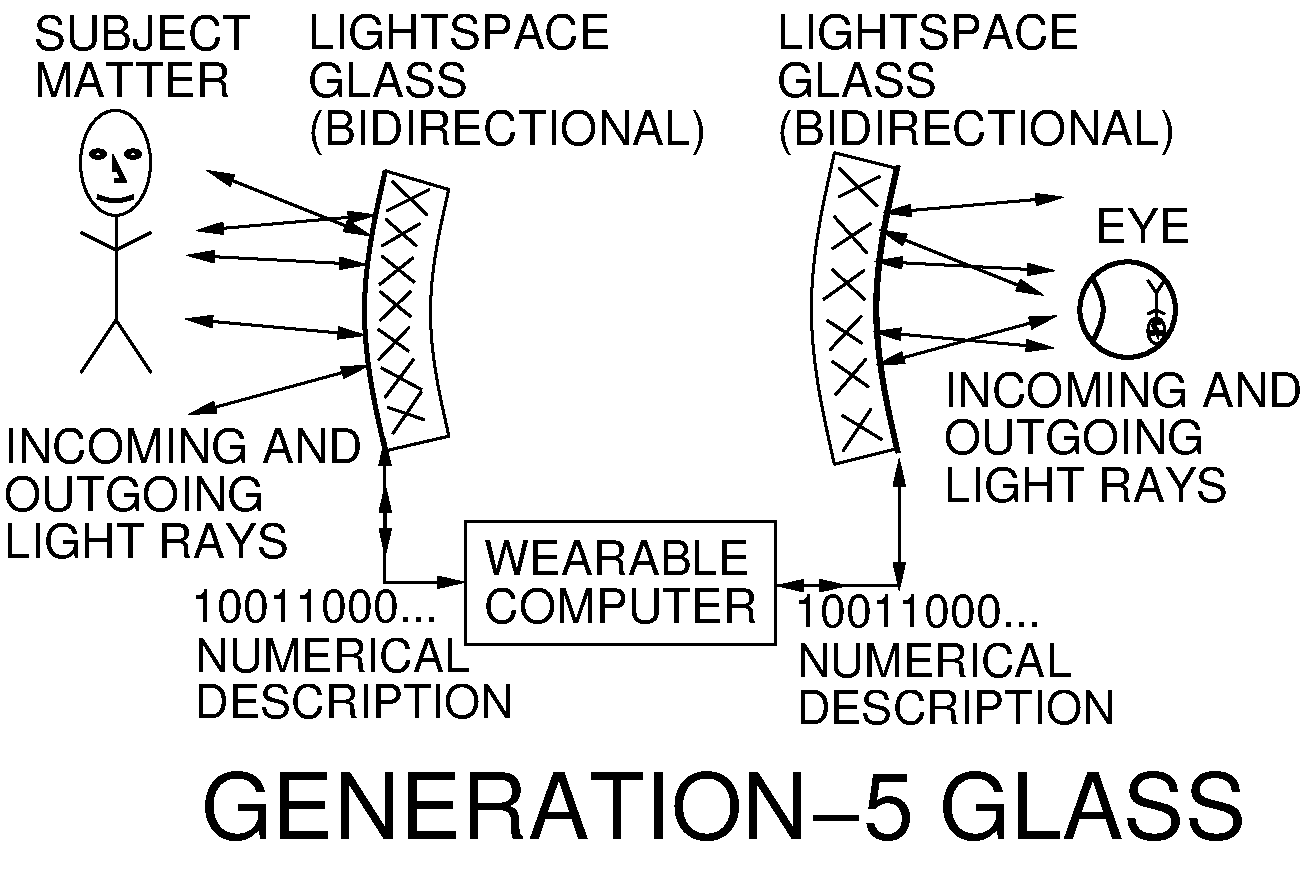
\includegraphics[width=3.75in]{ch6/figs/GL455.pdf}\\
  \caption{Proposed Generation-5 Glass.  Conceptually it is characterized
           by a bi-directional sensing and display modality.  Rays of light
           are sensed from BOTH THE SCENE AND THE EYE.  This facilitates
           eye-tracking as well as scene analysis. Computer-generated rays of light are also sent to 
BOTH THE
           EYE AND THE SCENE to facilitate active vision as well as
           being able to display content to other people who are not wearing
           the glass~\cite{mann2013freeglass}.}
  \label{fig:genfive}
\end{figure}

The development of the Gen-5 Glass is the focus of this thesis, which aims to create a ubiquitous 
wearable computing platform that enables a truly human-centric, intuitive computing environment by 
providing seamless integration between the human and the computer.

The Gen-5 Glass computing platform consists of two major components:
\begin{itemize}
  \item a hardware arrangement that consists of true stereoscopic 3D display glass and a time-of-flight 
3D range-sensing camera.  Other accessory devices such as a
        miniature laser data projector, eye-tracker, inertia measurement units (IMU), and brain-computer 
interface   sensors are also attached;
  \item a sophisticated software environment that simulates the EyeTap
        principle.  Because the camera is a 3D camera, it captures spatial-tonal
        information, allowing its point-of-view to be re-rendered from a
        left Point-of-Eye for the left eye, and, separately, a
        right Point-of-Eye for the right eye of the wearer.
\end{itemize}

A number of technical challenges arose in the creation of the Gen-5 Digital Eye Glass system, 
including optics design, calibration and alignment, head tracking and gesture tracking, form factor, 
latency management, human-computer interaction techniques, and Humanistic Intelligence 
(HI)~\cite{azuma1997survey, azuma2001recent, mann2001wearable}  which has recently become an 
active area of research. Specifically, the Humanistic Intelligence (HI) 
Framework~\cite{mann2001wearable} brings forth various topics in design decision and a new form of 
intelligent signal processing which forms an important basis of this thesis. One profound aspect of HI 
is the understanding of how human (and the human brain) should be an integral part of the computer 
system to create the superhuman intelligence as shown in Fig.~\ref{fig:hiflow}. The creation of the 
synergy between human and computer, which is summarized in the quote by Kurzweil, Minsky, and 
Mann~\cite{minsky2013society} at the beginning of the chapter, has a significant implication on the 
future of wearable computing. In the following section, a detailed description of the HI theories, as well 
as the core focus of the thesis in extending human capabilities, will be described.

\section{Humanistic Intelligence Framework}
\label{hiframeworks}

Many of the inventions and advancements in technology have changed the way we communicate and 
how we interact with the world. For example, the ability to communicate wirelessly with a handheld 
device (such as a mobile phone) radically changed the way we share and exchange information in 
this society. Trillions of instant messages are being sent per year\footnote{Mobile message traffic 
worldwide in 2012 and 2017 (in trillions)~\url{https://www.statista.com/statistics/262005/mobile-
message-traffic-worldwide/}} and billions of images are being uploaded and shared across the world 
daily\footnote{Internet Trends 2016 - Code Conference~\url{http://www.kpcb.com/internet-trends}}. 
Meanwhile, the recent innovation in human-computer interfaces from multi-touch interfaces to 
augmented, virtual, mixed, or aug-mediated reality interfaces have further redefined how we interact 
with the real world and the digital world. Computers are becoming increasingly more capable as they 
are equipped with more sensors such as motion sensors, depth sensors, or biometric sensors, which 
allow computers to observe human and infer our behaviours in our everyday lives and to act as our 
``personal assistant". Inevitably, the future of wearable computing will be characterized by an 
extremely close synergy between humans and computers. A set of questions and research problems 
arise as computers and humans are no longer separate entities in the feedback loop, and these 
questions lead to the field of research in Humanistic Intelligence (HI). 

\begin{figure}[htb]
\center
 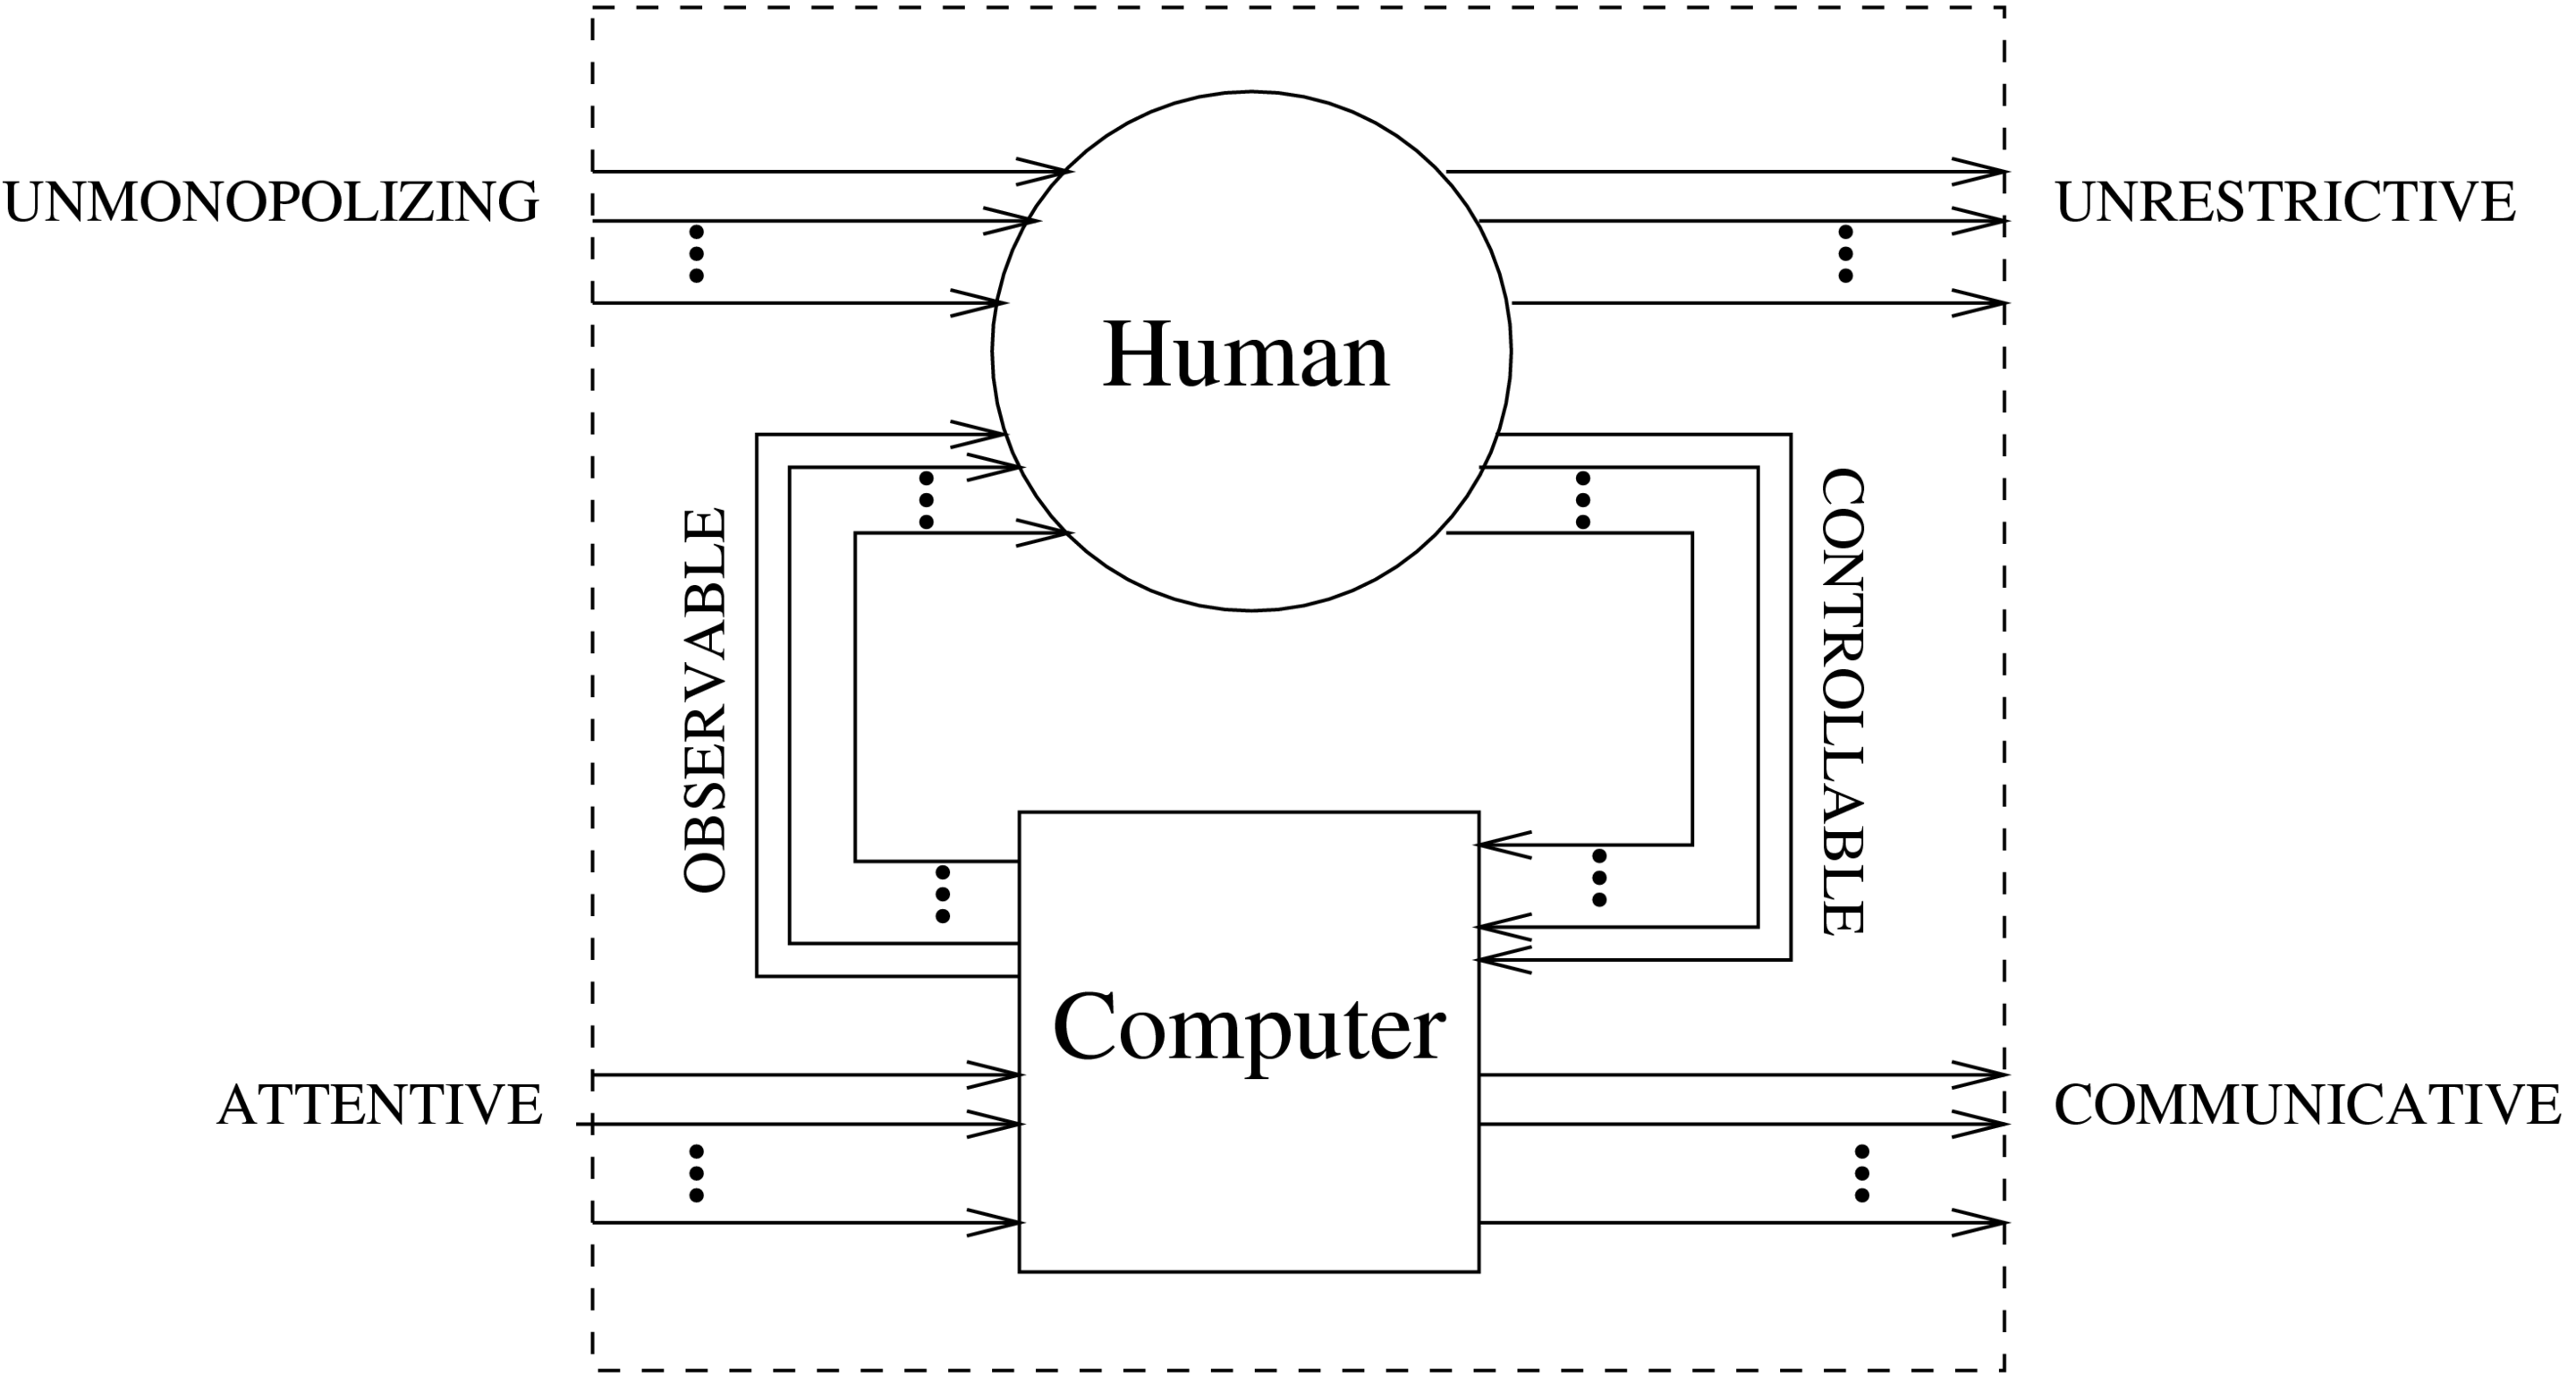
\includegraphics[width=6.0in]{ch1/figures/Humanistic_intelligence_wearcompdef_multichannel6only.png}
 \caption{The six signal flow paths in Humanistic Intelligence Framework. These six signal flow paths 
each defines one of the six attributes of WearComp~\cite{mann2001wearable}.}
 \label{fig:hiflow}
\end{figure}

One important aspect of HI is characterized by the processing hardware that is inextricably intertwined 
with a human being to function as a true extension of the user's mind and body. That is, the hardware 
is constant (`always ready'), provides augmentation (computing is NOT the primary task), and 
mediation (encapsulates the user). The notation of mediation is to create the ability to manage the 
information flow from the outside world, which creates a strong user empowerment tool.

The six basic signal flow paths of WearComp can be briefly summarized as follows 
(Fig.~\ref{fig:hiflow}): 

%REWRITE THIS SHIT....
\begin{enumerate}
   \item Unmonopolizing 
   \begin{itemize}
     \item The hardware does not isolate one from the outside world (e.g., replace the reality with a 
virtual world). Ideally, the WearComp device provides enhanced sensory capabilities. It may, however, 
facilitate mediation (augmenting, altering, or deliberately diminishing) of these sensory capabilities.  
   \end{itemize}
   \item Attentive
   \begin{itemize}
     \item The hardware has awareness of the environment with multi-modal and multi-sensory inputs. 
For example, one may want to combine a depth sensing camera, color camera, and perhaps fish eye 
camera to the system, and this ultimately gives the user increased situational awareness.
   \end{itemize}
   \item Unrestrictive
   \begin{itemize}
     \item The hardware is mobile and allows the user to perform other everyday tasks, e.g., one can 
give inputs to the system while walking down stairs or jogging without being restricted by the wearable 
system.
   \end{itemize}
   \item Communicative
   \begin{itemize}
     \item The hardware is used as a communication medium, as a means of assisting the user with the 
production of expressive or communicative media.
   \end{itemize}
   \item Observable
   \begin{itemize}
     \item The hardware provides user feedback continuously and is always observable within some 
reasonable limitations (e.g., the computer screen is not visible during the blinking of the eye).
   \end{itemize}
   \item Controllable
   \begin{itemize}
     \item The hardware is responsive and the user can take control over any part of the system when 
necessary. Any automated process and control loop shall include manual override control at any 
moment. 
   \end{itemize}
\end{enumerate}


Among these criteria, the key limiting factor in the realization of aug-mediated reality is that the 
experience enabled by the system can only be as good as the components used to create it. The 
limited dynamic range of the sensors, in particular, had hindered the Digital Eye Glass to be 
ubiquitously adopted in many situations. The lack of dynamic range of the sensor creates many ``blind 
spots'' or failure modes in a real world scene where the user and the computer may fail to see clearly. 
Thus, one key objective of this thesis is to address these shortcomings, and provide a real-time 
solution which pushes the boundary of the research on high dynamic range imaging.


\section{Mediation and Seeing Beyond}
As stated by Mann~\cite{mann2001wearable}, the most fundamental paradigm shift that WearComp 
has to offer is that of personal empowerment through the ability to individual with a personalized, 
customizable information space which is owned, operated, and controlled by the wearer. To realize 
the WearComp principles, especially on augmentation and mediation, we need to address the 
fundamental hardware and software limitations on the apparatus itself. One of the limiting factors in 
the design of the Digital Eye Glass is the lack of dynamic range in the camera sensors. Without a 
sufficient dynamic range, the person wearing the Digital Eye Glass would not be able to capture the 
true visual experience, and the computers cannot detect the salient features that provide reliable 
tracking. The notion of high dynamic range (HDR) video processing in the context of wearable 
computing is particularly attractive, as it would further augment and mediate (aug-mediate) our ability 
to see, even beyond the natural limits imposed by the human eye.  Furthermore, the limited dynamic 
range of the human eye presents significant challenges in our ability to see clearly in situations such 
as low-light conditions and/or high contrast scenes. 

For example, in welding, it is often necessary to wear protective eyewear such as a darkening helmet 
to prevent damage from the bright light. Unfortunately, with the helmet, one would not be able to see 
the scene clearly, which can impose great danger to the worker.  However, with HDR-based Digital 
Eye Glass, we would be able to overcome this problem by intelligently processing scenes with 
extremely high dynamic range for display in a human-sensible range.  Additionally, with 3D sensors, 
we could further provide a true sense of depth so that the Digital Eye Glass can truly become an 
integral part of the human experience.  This thesis explores methods to address the fundamental 
limitations of human vision, namely the limited dynamic range and depth sensing capability. In 
addition, novel real-time applications of the Digital Eye Glass in high dynamic range environment are 
presented.

\subsection{High Dynamic Range Imaging}
Despite recent advances in camera sensing technology, state-of-the-art digital cameras can only 
sense a limited dynamic range -- much less than the human eye. This limitation is particularly 
pronounced when viewing an extreme dynamic range scene, such as looking at the license plate 
number while being blinded by the headlights of a car on the other side of a dark road, or while doing 
electric arc welding.

Previous work over the last 25 years has focused on overcoming this limitation by combining 
differently exposed images of the same subject matter to generate High Dynamic Range (HDR) 
images~\cite{mannist}. 

As  Robertson et al.\ stated~\cite{robertson2003estimation}:
\begin{quote}
  ``The first report of digitally combining multiple pictures of the
  same scene to improve dynamic range appears to be
  Mann~\cite{mannist}''.
\end{quote} 

Over the past decade, HDR imaging has gained significant interest and numerous solutions have 
been proposed to create high quality HDR 
images~\cite{mannist,comparam,robertson2003estimation,debevec2008recovering}
and videos~\cite{kang2003high,ali2012ICASSP,irawan2005perceptually, HDRVideoCamera11}.
However, very little focus has been put into real-time algorithms that can
allow real-time interaction with the world.  Furthermore, the ability to run
at interactive frame rates is particularly important for the development of
HDR seeing aids~\cite{mann2004continuous} which can allow people to see in
extreme dynamic range conditions, where humans would not be able to {\em see}
with the naked eye, especially in the elderly or those with mild visual impairment.

\section{Thesis Organization and Overview}
This thesis emphasizes on the development of the EyeTap Aug-mediated Reality Digital Eye Glass 
system to address the fundamental limitations of human vision and our sensory capability, namely the 
limited dynamic range, the depth sensing abilities in 3D, and the limited ability in detecting 
phenomena outside of our detectable spectrum (e.g., seeing in the infrared or ultraviolet). In particular, 
a real-time application of the Digital Eye Glass in an HDR environment was developed in the most 
extreme dynamic range scene: tungsten inert gas (TIG) welding.  In addition, the work was extended 
with the use of 3D range sensing cameras which compute depth information with structured light 
patterns to enable gesture control in real-time.  Rather than using 3D range cameras to look at the 
user as used conventionally, the situation is reversed by mounting them on the user's head, thereby 
enabling human-centric wearable applications such as navigation, gesture recognition, and 
Lifelogging (cyborglogging)~\cite{mann2006cyborglogging,benedikt2015dagstuhl, billinghurst2015augmenting,gurrin2014lifelogging} as a visual memory prosthetic. Finally, this thesis discusses the social implications of the technology when 
3D-HDR-enabled Digital Eye Glass is worn to become an integral part of our daily life.

Various iterations of the Digital Eye Glass presented in this thesis were designed, prototyped, and 
worn by me and many others in their daily lives. These collective experiences framed the core 
learning component of this thesis and also formed the basis for the practical embodiment of the 
proposed HI framework. By continuously wearing, prototyping, and advancing the Digital Eye Glass, a 
set of observations, particularly those related to human-computer interaction, emerged. Here, I will 
discuss the realization of the core principles in the Humanistic Intelligence (HI) framework in practice 
and how multiple directions of research were taken. 


\textbf{Chapter~\ref{realtimehdrfpgas}} presents the first embodiment of the real-time implementation 
of the Digital Eye Glass system. This implementation explores the design of wearable eyeglasses 
system which addresses the dynamic range management problem (unmonopolized, observable and 
controllable attributes in HI). This chapter addresses the real-time component by implementing the 
system in a hardware-accelerated platform such as FPGAs and GPUs and discusses various key 
contributions in the HDR composition methods and hardware-accelerated tone mapping algorithms. 
Both approaches showed significant speed up, and fulfilled the requirements of an HI computing 
device. A set of applications demonstrating the use of this real-time HDR Digital Eye Glass system in 
our everyday life are also presented.
 
\textbf{Chapter~\ref{3dhdr3dsensing}} addresses the fundamental limitations of 3D sensing with a 
novel way of combining multiple exposure of 3D depth data by leveraging the work in 
\textbf{Chapter~\ref{realtimehdrfpgas}}. This approach demonstrates how one can design a high 
dynamic range (range in depth) sensor with simultaneous exposures with multiple depth sensors. At 
the time of publication, it was the first known approach which enhances both tonal range and spatial 
range in 3D space. The proposed algorithm provides a simple, yet effective way to calibrate and 
create a 3D HDR scene in real-time, and is ideal for wearable use cases where the environment is 
often unknown.
 
\textbf{Chapter~\ref{ar3dgesture}} presents the design of a depth sensing based Digital Eye Glass 
device, providing the first step toward a truly intelligent system in our everyday life. The result is a fully 
untethered, wearable Digital Eye Glass that also performs tasks with natural gesture inputs 
(augmentation of our everyday life). This device also enables night vision, and can function as a 
seeing aid, and as a range finder. The design principles in the HI framework were fully realized in the 
setup (e.g., observable (constancy) and controllable) and become a true extension of the body and 
mind. With the long-term use of such a device, the user often acquires a new skill with their existing 
senses. For example, the improvement in distance estimation can be achieved by training with the 3D 
range finder which suggests a potential realization of \textit{superhuman} intelligence with HI 
principles.

Finally, \textbf{Chapter~\ref{freeglassdevelopers}} demonstrates the use of the Digital Eye Glass in a 
social setting and its broader implications in the society with its wide adoption in the future. This 
chapter also illustrates various other applications and discusses the topic of sur/sous-veillance which 
arises in the development of the Digital Eye Glass for widespread use in our society.



